% Options for packages loaded elsewhere
\PassOptionsToPackage{unicode}{hyperref}
\PassOptionsToPackage{hyphens}{url}
\PassOptionsToPackage{dvipsnames,svgnames,x11names}{xcolor}
%
\documentclass[
  10pt,
]{article}
\usepackage{amsmath,amssymb}
\usepackage{iftex}
\ifPDFTeX
  \usepackage[T1]{fontenc}
  \usepackage[utf8]{inputenc}
  \usepackage{textcomp} % provide euro and other symbols
\else % if luatex or xetex
  \usepackage{unicode-math} % this also loads fontspec
  \defaultfontfeatures{Scale=MatchLowercase}
  \defaultfontfeatures[\rmfamily]{Ligatures=TeX,Scale=1}
\fi
\usepackage{lmodern}
\ifPDFTeX\else
  % xetex/luatex font selection
\fi
% Use upquote if available, for straight quotes in verbatim environments
\IfFileExists{upquote.sty}{\usepackage{upquote}}{}
\IfFileExists{microtype.sty}{% use microtype if available
  \usepackage[]{microtype}
  \UseMicrotypeSet[protrusion]{basicmath} % disable protrusion for tt fonts
}{}
\makeatletter
\@ifundefined{KOMAClassName}{% if non-KOMA class
  \IfFileExists{parskip.sty}{%
    \usepackage{parskip}
  }{% else
    \setlength{\parindent}{0pt}
    \setlength{\parskip}{6pt plus 2pt minus 1pt}}
}{% if KOMA class
  \KOMAoptions{parskip=half}}
\makeatother
\usepackage{xcolor}
\usepackage{longtable,booktabs,array}
\usepackage{calc} % for calculating minipage widths
% Correct order of tables after \paragraph or \subparagraph
\usepackage{etoolbox}
\makeatletter
\patchcmd\longtable{\par}{\if@noskipsec\mbox{}\fi\par}{}{}
\makeatother
% Allow footnotes in longtable head/foot
\IfFileExists{footnotehyper.sty}{\usepackage{footnotehyper}}{\usepackage{footnote}}
\makesavenoteenv{longtable}
\usepackage{graphicx}
\makeatletter
\def\maxwidth{\ifdim\Gin@nat@width>\linewidth\linewidth\else\Gin@nat@width\fi}
\def\maxheight{\ifdim\Gin@nat@height>\textheight\textheight\else\Gin@nat@height\fi}
\makeatother
% Scale images if necessary, so that they will not overflow the page
% margins by default, and it is still possible to overwrite the defaults
% using explicit options in \includegraphics[width, height, ...]{}
\setkeys{Gin}{width=\maxwidth,height=\maxheight,keepaspectratio}
% Set default figure placement to htbp
\makeatletter
\def\fps@figure{htbp}
\makeatother
\setlength{\emergencystretch}{3em} % prevent overfull lines
\providecommand{\tightlist}{%
  \setlength{\itemsep}{0pt}\setlength{\parskip}{0pt}}
\setcounter{secnumdepth}{5}

\usepackage{amsmath,amssymb}
\usepackage{graphicx}
\usepackage{longtable,booktabs,array}
\usepackage{xcolor}
\usepackage[margin=2.1cm]{geometry}
\usepackage{microtype}
\setlength{\emergencystretch}{3em}
\pdfinfoomitdate=1
\pdftrailerid{}
\pdfsuppressptexinfo=-1
\renewcommand{\arraystretch}{1.15}
\allowdisplaybreaks
\ifLuaTeX
  \usepackage{selnolig}  % disable illegal ligatures
\fi
\IfFileExists{bookmark.sty}{\usepackage{bookmark}}{\usepackage{hyperref}}
\IfFileExists{xurl.sty}{\usepackage{xurl}}{} % add URL line breaks if available
\urlstyle{same}
\hypersetup{
  pdftitle={UM-2: a 4+4 model of the Universe},
  pdfauthor={Underlying theory: Patrick L. Nash; Derived and verified by Claude (Anthropic); Model definition, version 1, 2026-10-17; Repository once-ere/Dirac\_claude, folder universe\_model\_2},
  colorlinks=true,
  linkcolor={blue},
  filecolor={Maroon},
  citecolor={Blue},
  urlcolor={blue},
  pdfcreator={LaTeX via pandoc}}

\title{UM-2: a 4+4 model of the Universe}
\usepackage{etoolbox}
\makeatletter
\providecommand{\subtitle}[1]{% add subtitle to \maketitle
  \apptocmd{\@title}{\par {\large #1 \par}}{}{}
}
\makeatother
\subtitle{Einstein-Lovelock gravity, the dirac16complex field, photons,
neutrinos, electrons, up and down quarks, gluons, and the \(W^+\),
\(W^-\) and \(Z\) bosons without a Higgs particle; every mass from the
\(x_0\) dependence of wave functions}
\author{Underlying theory: Patrick L. Nash \and Derived and verified by
Claude (Anthropic) \and Model definition, version 1,
2026-10-17 \and Repository once-ere/Dirac\_claude, folder
universe\_model\_2}
\date{}

\begin{document}
\maketitle

{
\hypersetup{linkcolor=}
\setcounter{tocdepth}{3}
\tableofcontents
}
\hypertarget{how-to-read-this-document}{%
\section{How to read this document}\label{how-to-read-this-document}}

This document DEFINES the model UM-2. Every field, every interaction and
every equation of the model is written out here; nothing has to be
looked up elsewhere. Each statement carries one of these labels:

\begin{itemize}
\tightlist
\item
  \textbf{DERIVED}: computed and verified in this work (sympy or
  numerics; the verification is stated with the result);
\item
  \textbf{AUTHOR}: taken from the author's notebooks (coordinates,
  metric, Lovelock weights, gamma matrices, mass parameter);
\item
  \textbf{STANDARD}: textbook physics used as an input;
\item
  \textbf{ASSUMED}: a choice made for this model;
\item
  \textbf{INVENTED}: a new phenomenological ingredient of this model;
\item
  \textbf{OPEN}: not resolved in this version.
\end{itemize}

Units: \(\hbar = c = 1\) unless stated. Indices \(M, N, \dots\) run over
the eight coordinates, \(a, b, \dots\) over the orthonormal frame,
\(\mu, \nu\) over the four observable coordinates
\(x_1, x_2, x_3, x_4\).

\hypertarget{summary}{%
\section{Summary}\label{summary}}

\begin{enumerate}
\def\labelenumi{\arabic{enumi}.}
\tightlist
\item
  \textbf{Spacetime.} Eight dimensions with the author's coordinates
  \(X = \{x_0, x_1, x_2, x_3, x_4, x_5, x_6, x_7\}\): \(x_0\) is the
  hidden space-like direction, \(x_1, x_2, x_3\) are ordinary space,
  \(x_4\) is the time, and \(x_5, x_6, x_7\) are three extra time-like
  directions. The frame metric is
  \(\eta = \mathrm{diag}(+1,+1,+1,+1,-1,-1,-1,-1)\) in this order. The
  metric depends on \(x_0\) only through \(z = 6Hx_0\) with period
  \(\pi\) in \(z\), i.e.~period \(\ell_0 = \pi/(6H)\) in \(x_0\).
\item
  \textbf{Gravity.} Einstein-Lovelock gravity in eight dimensions with
  the author's weights \(w = (1, 1/32, 1/1152)\) and
  \(\Lambda = -10H^2\), kept unchanged. A block stabiliser (a vacuum
  energy of the hidden block, ASSUMED) gives a stable static block at
  \(k_* = 12 + \tfrac43\sqrt{51}\) on which four-dimensional gravity is
  attractive: its Einstein-Hilbert coefficient is
  \(G(k_*) = \tfrac{20}{3} + \sqrt{51} = 13.81 > 0\) (DERIVED).
\item
  \textbf{The deflating extra times.} In the primordial era the extra
  times \(x_5, x_6, x_7\) (and \(x_0\) with them) deflate at rates up to
  \(2.6H\) into the stabilised block, then the block oscillates with the
  radion frequency \(3.387H\) while 3-space keeps expanding (DERIVED,
  full nonlinear equations).
\item
  \textbf{dirac16complex} \(\Psi\): a 16-component complex anticommuting
  spinor of \(Cl(4,4)\) (Pin(4,4) irreducible; two inequivalent
  8-dimensional irreducible representations of Spin(4,4)) coupled to
  gravity through the canonical spin connection, which is non-trivial:
  \(\gamma^M\Omega_M = \tfrac32(H/f)\gamma^{x_0} + (\dot b_4/b_4 - \tfrac12\dot a_4)\gamma^{x_4}\).
  It splits into two Lorentz-invariant halves, \(\Psi_A\) (\(B = -1\))
  and \(\Psi_B\) (\(B = +1\)), with \(B = -iC\gamma^{x_4}\) the Krein
  metric.
\item
  \textbf{Standard-Model content (one generation, no Higgs particle).}
  Photon, gluons, \(W^+\) (charge \(+e\)), \(W^-\) (charge \(-e\)),
  \(Z\) (neutral), the electron, one neutrino, the up and down quarks
  (confined into protons and neutrons). Electroweak symmetry is broken
  at the regular tip of the hidden direction by a non-linear sigma field
  \(\Sigma \in SU(2)\) that has no radial mode, hence no Higgs particle.
\item
  \textbf{Masses.} Every four-dimensional mass is the eigenvalue of an
  \(x_0\) operator acting on a wave function periodic in \(x_0\) with
  period \(\pi/(6H)\). Massless: graviton, photon, gluons (flat \(x_0\)
  profiles) and the fold band of \(\Psi\) (chiral zero modes). Massive:
  \(W^\pm\), \(Z\) (profiles bent at the tip), \(e\), \(\nu\), \(u\),
  \(d\) (chiral zero modes mixed at the tip), the bulk band of \(\Psi\)
  and every Kaluza-Klein mode (DERIVED spectra, fitted to the measured
  masses with order-one parameters).
\item
  \textbf{New interactions (INVENTED).} A chiral tip \(Z\) portal makes
  the \(\Psi_A\) fold band behave as two extra neutrino species, so that
  the \(Z\) invisible width (\(N_\nu = 2.984\)) is reproduced and
  \(N_{eff} = 3.044\) follows; a gauge-kinetic portal couples \(\Psi\)
  to pairs of gauge bosons (\(W^+W^-\), \(ZZ\), \(Z\gamma\),
  \(\gamma\gamma\), gluon pairs); a bounded vector contact portal
  couples \(\Psi\) to the fermion currents.
\item
  \textbf{The dark sector.} The lightest odd state of \(\Psi_B\), a
  Dirac fermion of mass \(3.1022\,m = 44.3\) TeV (\(m = H\)), is
  electrically and weakly neutral at tree level (exactly), stable by the
  fold parity, cold, and a dark-matter candidate. No state of \(\Psi\)
  is dark energy; the dark energy of UM-2 is a tuned four-dimensional
  cosmological term.
\item
  \textbf{Cosmology.} The four-dimensional effective theory of the
  stabilised block is exact general relativity, so the CMB, the CNB and
  the BAO follow from the standard Einstein-Boltzmann equations with the
  UM-2 particle content.
\end{enumerate}

\hypertarget{space-coordinates-and-the-periodic-hidden-direction}{%
\section{Space, coordinates and the periodic hidden
direction}\label{space-coordinates-and-the-periodic-hidden-direction}}

\hypertarget{the-coordinates-author}{%
\subsection{The coordinates (AUTHOR)}\label{the-coordinates-author}}

The author's coordinates are
\(X = \{x_0, x_1, x_2, x_3, x_4, x_5, x_6, x_7\}\) (the author's
notebook: \texttt{X\ =\ \{x0{[}{]},\ x1{[}{]},\ ...,\ x7{[}{]}\}}), with

\begin{itemize}
\tightlist
\item
  \(x_0\): the hidden space-like direction, \(z \equiv 6Hx_0\) takes
  every real value;
\item
  \(x_1, x_2, x_3\): ordinary 3-space;
\item
  \(x_4\): the time;
\item
  \(x_5, x_6, x_7\): three extra time-like directions.
\end{itemize}

\(H > 0\) is the author's constant. Frame indices \(a = 0, \dots, 7\)
are aligned with \(x_0, \dots, x_7\), and
\[\eta_{ab} = \mathrm{diag}(+1, +1, +1, +1, -1, -1, -1, -1).\]

\hypertarget{the-hidden-coordinate-y-the-fold-and-the-tips-derived}{%
\subsection{\texorpdfstring{The hidden coordinate \(y\), the fold and
the tips
(DERIVED)}{The hidden coordinate y, the fold and the tips (DERIVED)}}\label{the-hidden-coordinate-y-the-fold-and-the-tips-derived}}

On every interval of \(z\) on which \(\sin z \neq 0\) define
\[ y = \frac{\ln|\sin z|}{6H} \in (-\infty, 0], \qquad |\sin z| = e^{6Hy}, \qquad dy = \cot z\, dx_0 .\]
One period \(0 < z < \pi\) of \(x_0\) (length \(\ell_0 = \pi/(6H)\))
consists of two halves, \(0 < z < \pi/2\) and \(\pi/2 < z < \pi\),
joined at the \textbf{fold} \(z = \pi/2\) (\(y = 0\), where
\(\cos z = 0\)). Each half ends at a \textbf{tip} (\(z \to 0^+\) or
\(z \to \pi^-\), \(y \to -\infty\)), at infinite proper distance from
the fold. As in the Kohn-Sham record of this repository the tip is
replaced by a regular cutoff at \(y = -L\) (ASSUMED), with
\[ \eta \equiv HL = 3 .\] The fold reflection
\[ R:\quad z \mapsto \pi - z \qquad (x_0 \mapsto \ell_0 - x_0)\] maps
the two halves onto each other; modes of a field on one period are even
or odd under \(R\). Every function of \(y(z)\) is periodic in \(x_0\)
with period \(\ell_0 = \pi/(6H)\).

\hypertarget{the-metric-as-a-power-series}{%
\section{The metric as a power
series}\label{the-metric-as-a-power-series}}

The metric is a series of terms of decreasing magnitude,
\[ g_{MN} = \bar g_{MN} + \epsilon\, h^{(1)}_{MN} + \epsilon^2 h^{(2)}_{MN} + \dots, \qquad \epsilon \sim 10^{-5}, \]
where \(\epsilon\) is the size of the CMB temperature anisotropy
(STANDARD).

\hypertarget{order-0-the-corrected-primordial-metric-author-coordinates-derived-properties}{%
\subsection{Order 0: the corrected primordial metric (AUTHOR
coordinates, DERIVED
properties)}\label{order-0-the-corrected-primordial-metric-author-coordinates-derived-properties}}

In the author's chart, with two general functions of the time
\(a_4(x_4)\) and \(b_4(x_4) > 0\),
\[ \bar g = \mathrm{diag}\Big( e^{-2a_4} b_4 \cot^2 z,\; e^{2a_4},\; e^{2a_4},\; e^{2a_4},\; -1,\;
   -e^{-2a_4} b_4 (\sin^2 z)^{1/6},\; -e^{-2a_4} b_4 (\sin^2 z)^{1/6},\; -e^{-2a_4} b_4 (\sin^2 z)^{1/6} \Big), \]
where \((\sin^2 z)^{1/6}\) is the positive branch. This is the metric of
the Revision record of 2026-10-16 (version 2), whose sources are all
diagonal. The notebook metric
\[ \begin{aligned} g^{\text{nb}} = \mathrm{diag}\big(&\cot^2 z,\; e^{2a_4}(\sin^2z)^{1/6},\; e^{2a_4}(\sin^2z)^{1/6},\; e^{2a_4}(\sin^2z)^{1/6},\\
   &-1,\; -e^{-2a_4}(\sin^2z)^{1/6},\; -e^{-2a_4}(\sin^2z)^{1/6},\; -e^{-2a_4}(\sin^2z)^{1/6}\big), \end{aligned} \]
to whose extra-time components the author's order of 2026-10-14 added
the factor \(b_4\), differs from it in \(g_{00}\) and in the 3-space
warp. Define
\[ f = e^{-a_4} b_4^{1/2}, \qquad k = \frac{1}{f^2} = \frac{e^{2a_4}}{b_4}, \qquad A = \dot a_4, \qquad h = \frac{\dot f}{f} = \frac{\dot b_4}{2b_4} - \dot a_4 , \]
dots being \(d/dx_4\). In the \(y\) chart the metric is
\[ d\bar s^2 = e^{2a_4}(dx_1^2 + dx_2^2 + dx_3^2) - dx_4^2 + f^2\big[dy^2 - e^{2Hy}(dx_5^2 + dx_6^2 + dx_7^2)\big] .\]
The block \(\{x_0, x_5, x_6, x_7\}\) is \(f^2\) times a four-dimensional
space of constant curvature \(-H^2\) and signature \((1,3)\); \(f\) is
its common scale factor (``the block''), \(A\) is the observer's Hubble
rate and \(h < 0\) means that the extra times and \(x_0\) deflate. The
volume element and the vielbein are
\[ \sqrt{|\bar g|} = e^{3a_4} f^4\, |\cot z|\,(\sin^2 z)^{1/4} = e^{3a_4} f^4 e^{3Hy}\,\Big|\frac{dy}{dx_0}\Big| ,\]
\[ e^0{}_{x_0} = f\cot z,\quad e^i{}_{x_i} = e^{a_4}\ (i = 1,2,3),\quad e^4{}_{x_4} = 1,\quad e^t{}_{x_t} = f(\sin^2 z)^{1/12}\ (t = 5,6,7) .\]

\textbf{Curvature (DERIVED; sympy, identical in both charts, 25/25
checks).} The Riemann tensor is pair-diagonal, \(R^{ab}{}_{cd} = 0\)
unless \(\{a,b\} = \{c,d\}\), and every sectional curvature
\(K_{ab} = R^{ab}{}_{ab}\) is one of
\[ K_{ij} = A^2,\quad K_{i4} = A^2 + \dot A,\quad K_{iB} = A h,\quad K_{4B} = h^2 + \dot h,\quad K_{BB'} = h^2 - H^2 k, \]
with \(i, j \in \{1,2,3\}\) and \(B, B' \in \{0,5,6,7\}\). None depends
on \(x_0\); the curvature is the same on both halves of every period.

\hypertarget{order-1-the-observable-perturbations-and-the-hidden-tower}{%
\subsection{Order 1: the observable perturbations and the hidden
tower}\label{order-1-the-observable-perturbations-and-the-hidden-tower}}

Every field and every metric perturbation is expanded in the
eigenfunctions \(u_n(x_0)\) of its \(x_0\) operator (section 6),
\[ h^{(1)}_{MN}(x^\mu, x_0) = \sum_{n \ge 0} h^{(1,n)}_{MN}(x^\mu)\, u_n(x_0). \]
The \(n = 0\) term has the flat profile \(u_0 = \text{const}\); in the
Newtonian gauge its line element is
\[ ds^2 = e^{2a_4}\big[(1 - 2\epsilon\Psi_N)\delta_{ij} + \epsilon h^{TT}_{ij}\big]dx_i dx_j - (1 + 2\epsilon\Phi)dx_4^2
   + f^2(1 + 2\epsilon\sigma)\big[dy^2 - e^{2Hy}dx_t^2\big], \] with the
two scalar potentials \(\Phi\), \(\Psi_N\), the transverse-traceless
tensor \(h^{TT}_{ij}\) and the radion \(\sigma\) (the relative
fluctuation of the block size). The scalar and tensor sectors carry the
CMB, the CNB and the BAO; the radion is massive (section 8.3) and does
not propagate at cosmological distances. The terms \(n \ge 1\) are
Kaluza-Klein modes with masses above the gap \(3H/(2f)\) (section 6).
Order 2 contains the products of order-1 terms and the back-reaction of
\(x_0\)-localised sources; it is not computed in this version (OPEN).

\hypertarget{the-action}{%
\section{The action}\label{the-action}}

\[ S = S_{EL}[g] + S_{stab}[g] + S_\Psi[g, \Psi] + S_{gauge}[g, G, W, B] + S_{f}[g, \psi; G, W, B] + S_{tip}[g; W, B, \Sigma, \psi]
   + S_{portal}[\Psi; \psi, G, W, B, \Sigma] . \]

\hypertarget{einstein-lovelock-gravity-author-weights}{%
\subsection{Einstein-Lovelock gravity (AUTHOR
weights)}\label{einstein-lovelock-gravity-author-weights}}

\[ S_{EL} = \frac{1}{2\kappa}\int d^8x\,\sqrt{|g|}\,\Big(\sum_{k=1}^{3}\alpha_k\,\mathcal L_{(k)} - 2\Lambda\Big), \qquad
   \mathcal L_{(k)} = \frac{1}{2^k}\,\delta^{a_1b_1\cdots a_kb_k}_{c_1d_1\cdots c_kd_k}\,
   R^{c_1d_1}{}_{a_1b_1}\cdots R^{c_kd_k}{}_{a_kb_k}, \] with the
generalised Kronecker delta \(\delta^{\cdots}_{\cdots}\) (the
determinant of ordinary deltas). \(\mathcal L_{(1)} = R\),
\(\mathcal L_{(2)} = R^2 - 4R_{ab}R^{ab} + R_{abcd}R^{abcd}\)
(Gauss-Bonnet) and \(\mathcal L_{(3)}\) is the cubic Lovelock density.
The field equations are
\[ \sum_{k=1}^{3}\alpha_k\,E_{(k)}{}^M{}_N + \Lambda\,\delta^M_N = \kappa\,T^M{}_N, \qquad
   E_{(k)}{}^M{}_N = -\frac{1}{2^{k+1}}\,\delta^{M a_1 b_1\cdots a_k b_k}_{N c_1 d_1\cdots c_k d_k}\,
   R^{c_1d_1}{}_{a_1b_1}\cdots R^{c_kd_k}{}_{a_kb_k}, \] \(E_{(1)}\)
being the Einstein tensor. The author's weights are
\[ \alpha_k = w_k H^{2-2k}, \qquad w = (w_1, w_2, w_3) = \Big(1, \frac{1}{32}, \frac{1}{1152}\Big), \qquad \Lambda = -10H^2 \]
(the author's notebook writes \(\Lambda = 10\) with the opposite sign
convention for \(\Lambda\)). UM-2 keeps these values.

\textbf{For a pair-diagonal curvature (DERIVED).} When \(R^{ab}{}_{cd}\)
is pair-diagonal (the order-0 metric),
\[ \mathcal L_{(k)} = 2^k k! \sum_{\text{k disjoint pairs}}\ \prod_{\text{pairs}} K_{ab}, \qquad
   E_{(k)}{}^h{}_h = -2^{k-1} k!\!\!\sum_{\text{k disjoint pairs avoiding } h}\ \prod_{\text{pairs}} K_{ab}, \]
which was checked against the Einstein tensor from the Ricci tensor
(\(k = 1\)), against the explicit Gauss-Bonnet tensor (\(k = 2\)),
against the Bianchi identity \(\nabla_M E_{(k)}{}^M{}_N = 0\)
(\(k = 1, 2, 3\)), against the Euler-Lagrange equations of the action
with a lapse (\(k = 1, 2, 3\)) and against the record's equations (all
exact).

\hypertarget{the-block-stabiliser-assumed}{%
\subsection{The block stabiliser
(ASSUMED)}\label{the-block-stabiliser-assumed}}

A source term
\[ S_{stab} = -\int d^8x\,\sqrt{|g|}\;\rho_b(f), \qquad \kappa\,\rho_b(f) = \kappa\rho_b^*\Big(\frac{f_*}{f}\Big)^{8} ,\]
whose energy-momentum tensor is that of a vacuum energy of the block,
\[ T^M{}_N[\text{stab}] = \mathrm{diag}\big(p_0, p_3, p_3, p_3, -\rho_b, p_t, p_t, p_t\big), \qquad p_3 = -\rho_b, \qquad p_0 = p_t = +\rho_b .\]
It is conserved
(\(\dot\rho_b = -3A(\rho_b + p_3) - 4h(\rho_b + p_0) = -8h\rho_b\) gives
\(\rho_b \propto f^{-8}\)), it is four-dimensionally Lorentz invariant
(\(p_3 = -\rho_b\)) and isotropic in the block (\(p_0 = p_t\)), as the
field equations require (section 8.1), and it does not depend on
\(x_0\). The \(f^{-8}\) law is that of an eight-dimensional energy
density whose only scale is the size of the block (a Casimir-type or
flux energy). Its normalisation is fixed by the static block (section
8.2): \(\kappa\rho_b^* = (26 + 4\sqrt{51})H^2\) at \(f_* = k_*^{-1/2}\).
Its microscopic origin is OPEN (a Casimir energy of the fields of the
cell or a flux are natural candidates; neither was computed in UM-2).

\hypertarget{the-dirac16complex-field}{%
\subsection{The dirac16complex field}\label{the-dirac16complex-field}}

\hypertarget{the-clifford-algebra-of-the-author-author-derived-verification}{%
\subsubsection{The Clifford algebra of the author (AUTHOR, DERIVED
verification)}\label{the-clifford-algebra-of-the-author-author-derived-verification}}

The author's real \(16\times16\) matrices are built as follows
(\(h = 1, 2, 3\); \(p, q = 1, \dots, 4\); \(\epsilon\) the Levi-Civita
symbol; \(I_n\) the identity):
\[ Q_a(h,p,q) = \epsilon_{hpq4},\quad Q_b(h,p,q) = \delta_{p4}\delta_{qh} - \delta_{ph}\delta_{q4},\quad
   s_h = Q_a - Q_b,\quad t_h = Q_a + Q_b , \]
\[ \zeta_0 = I_8,\quad \zeta_{7-h} = \begin{pmatrix} 0 & t_h \\ -t_h & 0\end{pmatrix},\quad
   \zeta_h = \begin{pmatrix} 0 & s_h \\ s_h & 0\end{pmatrix},\quad \zeta_7 = \zeta_1\zeta_2\zeta_3\zeta_4\zeta_5\zeta_6,\quad
   \sigma = \begin{pmatrix} 0 & I_4 \\ I_4 & 0 \end{pmatrix}, \]
\[ \tau_0 = I_8,\quad \tau_A = \zeta_A\ (A = 1..7),\quad \bar\tau_A = \sigma\,\tau_A^{T}\sigma,\qquad
   \gamma^{x_A} \equiv T16[A] = \begin{pmatrix} 0 & \bar\tau_A \\ \tau_A & 0 \end{pmatrix}\quad (A = 0, \dots, 7). \]
They satisfy (DERIVED, exact; 31/31 checks)
\[ \{\gamma^a, \gamma^b\} = 2\eta^{ab} I_{16}, \qquad \tfrac12(\tau_A\bar\tau_B + \tau_B\bar\tau_A) = \eta_{AB}I_8,\qquad
   \sigma = \tau_1\tau_2\tau_3 = \tau_4\tau_5\tau_6\tau_7 . \] The
charge-conjugation matrix, the chirality, the Krein metric and the
generators are
\[ C = \gamma^{x_0}\gamma^{x_1}\gamma^{x_2}\gamma^{x_3} = \begin{pmatrix} -\sigma & 0 \\ 0 & \sigma\end{pmatrix},\quad
   \Gamma = \gamma^{x_0}\gamma^{x_1}\cdots\gamma^{x_7} = \mathrm{diag}(-I_8, I_8),\quad
   B = -iC\gamma^{x_4},\quad S^{ab} = \tfrac14[\gamma^a, \gamma^b], \]
with \(C^T = C\), \(C^2 = 1\), \((C\gamma^a)^T = -C\gamma^a\),
\(B^\dagger = B\), \(B^2 = 1\) and \(B\) of signature \((8,8)\). The
16-dimensional representation is irreducible under Pin(4,4) (commutant
of dimension 1), the double cover of \(O(4,4)\), and it splits under
Spin(4,4), the double cover of \(SO(4,4)\), into two inequivalent
irreducible 8-dimensional representations, the eigenspaces
\(\Gamma = \mp1\) (commutant of dimension 2, intertwiner of dimension
0).

\hypertarget{the-lagrangian-and-the-canonical-spin-connection}{%
\subsubsection{The Lagrangian and the canonical spin
connection}\label{the-lagrangian-and-the-canonical-spin-connection}}

\(\Psi\) has 16 complex anticommuting (Grassmann) components and
\(\bar\Psi = \Psi^\dagger C\). The Lagrangian density is
\[ \mathcal L_\Psi = \sqrt{|g|}\Big[\tfrac12\big(\bar\Psi\gamma^M D_M\Psi - (D_M\bar\Psi)\gamma^M\Psi\big) - m\,\bar\Psi\Psi - \tfrac{\lambda}{2}(\bar\Psi\Psi)^2\Big], \]
\[ \gamma^M = e_a{}^M\gamma^a,\quad D_M\Psi = \partial_M\Psi + \Omega_M\Psi,\quad D_M\bar\Psi = \partial_M\bar\Psi - \bar\Psi\Omega_M,\quad
   \Omega_M = \tfrac12\,\omega_{Mab}S^{ab}, \]
\[ \omega_M{}^a{}_b = e^a{}_N\big(\partial_M e_b{}^N + \Gamma^N{}_{ML}\,e_b{}^L\big),\qquad \omega_{Mab} = \eta_{ac}\,\omega_M{}^c{}_b , \]
the canonical (metric-compatible, torsion-free) spin connection: it
makes \(\gamma^N\) covariantly constant,
\(\partial_M\gamma^N + \Gamma^N{}_{ML}\gamma^L + [\Omega_M, \gamma^N] = 0\)
(DERIVED). For the order-0 metric (DERIVED, exact, for every \(a_4\),
\(b_4\) and on both halves)
\[ \gamma^M\Omega_M = \frac{3}{2}\,\frac{H}{f}\,\gamma^{x_0} + \Big(\frac{\dot b_4}{b_4} - \frac{\dot a_4}{2}\Big)\gamma^{x_4} ,\]
which vanishes only in flat 4+4 space (\(H = 0\) with constant \(a_4\),
\(b_4\)): the coupling of \(\Psi\) to gravity is non-trivial. The field
equation is
\[ \gamma^M D_M\Psi = \big(m + \lambda\,\bar\Psi\Psi\big)\Psi . \] The
mass parameter is the author's \(m = 3HM\); UM-2 uses \(M = 1/3\),
i.e.~\(m = H\) (ASSUMED, the value of the Kohn-Sham record). \(\lambda\)
(dimension mass\(^{-6}\)) is the contact self-coupling.

\hypertarget{the-two-halves-psi_a-and-psi_b-and-the-fold-parity-derived}{%
\subsubsection{\texorpdfstring{The two halves \(\Psi_A\) and \(\Psi_B\)
and the fold parity
(DERIVED)}{The two halves \textbackslash Psi\_A and \textbackslash Psi\_B and the fold parity (DERIVED)}}\label{the-two-halves-psi_a-and-psi_b-and-the-fold-parity-derived}}

\(B\) commutes with every four-dimensional Lorentz generator
\(\gamma^a\gamma^b\) (\(a, b \in \{x_1, .., x_4\}\)) and with \(C\), so
\[ \Psi = \Psi_A + \Psi_B, \qquad B\Psi_A = -\Psi_A, \qquad B\Psi_B = +\Psi_B \]
splits \(\Psi\) into two four-dimensionally Lorentz-invariant halves of
8 components, and \(\bar\Psi\Psi = \bar\Psi_A\Psi_A + \bar\Psi_B\Psi_B\)
does not mix them. In the good sector (no extra-time momenta) every
interaction of UM-2 commutes with \(B\) (DERIVED with the author's
matrices: \(B\) commutes with \(C\), \(\gamma^a\) and \(C\gamma^a\) for
\(a = x_0, \dots, x_4\) and anticommutes with them for
\(a = x_5, x_6, x_7\)), so the numbers \(N_A\) and \(N_B\) are
separately conserved; extra-time momenta would mix the halves. Under the
fold reflection \(R\) the modes are even or odd; the bulk Lagrangian is
\(R\)-symmetric.

\hypertarget{the-standard-model-gauge-fields-assumed-structure-standard-content}{%
\subsection{The Standard-Model gauge fields (ASSUMED structure, STANDARD
content)}\label{the-standard-model-gauge-fields-assumed-structure-standard-content}}

The gauge group is \(SU(3)_c\times SU(2)_L\times U(1)_Y\) with
eight-dimensional gauge fields \(G^\alpha_M\) (\(\alpha = 1..8\)),
\(W^a_M\) (\(a = 1, 2, 3\)) and \(B_M\):
\[ S_{gauge} = -\frac14\int d^8x\sqrt{|g|}\,g^{MP}g^{NQ}\Big(\frac{1}{\hat g_s^2}G^\alpha_{MN}G^\alpha_{PQ} + \frac{1}{\hat g^2}W^a_{MN}W^a_{PQ}
   + \frac{1}{\hat g'^2}B_{MN}B_{PQ}\Big), \]
\[ G^\alpha_{MN} = \partial_MG^\alpha_N - \partial_NG^\alpha_M + f^{\alpha\beta\gamma}G^\beta_MG^\gamma_N,\quad
   W^a_{MN} = \partial_MW^a_N - \partial_NW^a_M + \epsilon^{abc}W^b_MW^c_N,\quad B_{MN} = \partial_MB_N - \partial_NB_M . \]
The four-dimensional couplings are \(g_s^2 = \hat g_s^2/V_\perp\),
\(g^2 = \hat g^2/V_\perp\), \(g'^2 = \hat g'^2/V_\perp\), where
\(V_\perp\) is the proper volume of the block per unit 4-volume (section
7). In this geometric normalisation the couplings stand in front of the
kinetic terms and not in the covariant derivatives; the dimensions are
\([G_M] = [W_M] = [B_M] = 1\), \([\hat g^2] = -4\) (mass units), and the
four-dimensional couplings are dimensionless. From here on \(W^\pm\),
\(Z\), \(A\) and every formula that shows \(\hat g\), \(\hat g'\)
explicitly refer to the canonically normalised fields \(W^a/\hat g\),
\(B/\hat g'\), \(G^\alpha/\hat g_s\) (written with the same letters).
The physical fields are
\[ W^\pm_M = \frac{W^1_M \mp iW^2_M}{\sqrt2},\qquad Z_M = \cos\theta_W\,W^3_M - \sin\theta_W\,B_M,\qquad
   A_M = \sin\theta_W\,W^3_M + \cos\theta_W\,B_M,\qquad \tan\theta_W = \frac{g'}{g} . \]
\textbf{\(W^+\) carries the electric charge \(+e\) and \(W^-\) the
charge \(-e\)} (\([T_3, T_\pm] = \pm T_\pm\), \(Y(W) = 0\); \(W^-\) is
the antiparticle of \(W^+\)); \(Z\) and the photon \(A\) are neutral
(DERIVED). A fermion of weak isospin \(T_3\) and hypercharge \(Y\)
couples to \(A\) with \(e(T_3 + Y) = eQ\),
\(e = gg'/\sqrt{g^2 + g'^2}\), and to \(Z\) with
\(\sqrt{g^2 + g'^2}\,(T_3 - Q\sin^2\theta_W)\) (DERIVED). The
non-abelian terms of \(W^a_{MN}W^a_{PQ}\) contain the vertices
\(W^+W^-\gamma\) (strength \(e\)), \(W^+W^-Z\) (strength
\(g\cos\theta_W\)) and the quartic \(W^+W^-W^+W^-\),
\(W^+W^-\gamma\gamma\), \(W^+W^-Z\gamma\), \(W^+W^-ZZ\); every vertex
conserves electric charge, so a single \(W^+\) or \(W^-\) always comes
with a charged partner.

\hypertarget{the-standard-model-fermions-one-generation-assumed-structure-invented-boundary-assignment}{%
\subsection{The Standard-Model fermions (one generation; ASSUMED
structure, INVENTED boundary
assignment)}\label{the-standard-model-fermions-one-generation-assumed-structure-invented-boundary-assignment}}

Each multiplet is an eight-dimensional spinor of the same Clifford
algebra (16 components times its gauge indices):

\begin{longtable}[]{@{}
  >{\raggedright\arraybackslash}p{(\columnwidth - 10\tabcolsep) * \real{0.1667}}
  >{\raggedright\arraybackslash}p{(\columnwidth - 10\tabcolsep) * \real{0.1667}}
  >{\raggedright\arraybackslash}p{(\columnwidth - 10\tabcolsep) * \real{0.1667}}
  >{\raggedright\arraybackslash}p{(\columnwidth - 10\tabcolsep) * \real{0.1667}}
  >{\raggedright\arraybackslash}p{(\columnwidth - 10\tabcolsep) * \real{0.1667}}
  >{\raggedright\arraybackslash}p{(\columnwidth - 10\tabcolsep) * \real{0.1667}}@{}}
\toprule\noalign{}
\begin{minipage}[b]{\linewidth}\raggedright
field
\end{minipage} & \begin{minipage}[b]{\linewidth}\raggedright
\(SU(3)_c\)
\end{minipage} & \begin{minipage}[b]{\linewidth}\raggedright
\(SU(2)_L\)
\end{minipage} & \begin{minipage}[b]{\linewidth}\raggedright
\(Y\)
\end{minipage} & \begin{minipage}[b]{\linewidth}\raggedright
electric charges \(Q = T_3 + Y\)
\end{minipage} & \begin{minipage}[b]{\linewidth}\raggedright
4D zero mode
\end{minipage} \\
\midrule\noalign{}
\endhead
\bottomrule\noalign{}
\endlastfoot
\(Q = (u, d)_L\) & 3 & 2 & \(1/6\) & \(u\): \(2/3\), \(d\): \(-1/3\) &
\(\Gamma_4 = +1\) \\
\(u_R\) & 3 & 1 & \(2/3\) & \(2/3\) & \(\Gamma_4 = -1\) \\
\(d_R\) & 3 & 1 & \(-1/3\) & \(-1/3\) & \(\Gamma_4 = -1\) \\
\(L = (\nu, e)_L\) & 1 & 2 & \(-1/2\) & \(\nu\): 0, \(e\): \(-1\) &
\(\Gamma_4 = +1\) \\
\(e_R\) & 1 & 1 & \(-1\) & \(-1\) & \(\Gamma_4 = -1\) \\
\(\nu_R\) & 1 & 1 & 0 & 0 & \(\Gamma_4 = -1\) \\
\end{longtable}

with the action
\[ S_f = \sum_\psi\int d^8x\sqrt{|g|}\Big[\tfrac12\big(\bar\psi\gamma^MD_M\psi - (D_M\bar\psi)\gamma^M\psi\big) - \mu_\psi\bar\psi\psi\Big],\qquad
   D_M = \partial_M + \Omega_M - iG^\alpha_MT^\alpha - iW^a_M\frac{\tau^a}{2} - iY B_M , \]
the same canonical spin connection \(\Omega_M\) as for \(\Psi\) and a
constant bulk mass \(\mu_\psi\) per multiplet. The 4D chirality is
\(\Gamma_4 = i\gamma^{x_1}\gamma^{x_2}\gamma^{x_3}\gamma^{x_4}\).

\textbf{Boundary conditions.} In 16-component form, with the selection
projector
\[ P_{sel} = \frac{1 + \Gamma_4\gamma^{x_0}}{2}\,\frac{1 - i\gamma^{x_5}\gamma^{x_6}}{2}, \]
which commutes with every four-dimensional Lorentz generator (DERIVED),
the conditions at the fold (\(y = 0\)) and at the tip (\(y = -L\)) are

\begin{itemize}
\tightlist
\item
  doublets (\(Q\), \(L\); \(\mu_\psi > 0\)): fold
  \(P_{sel}(1 - \gamma^{x_0})\psi = 0\) and
  \((1 - P_{sel})(1 + \gamma^{x_0})\psi = 0\); tip
  \((1 - \gamma^{x_0})\psi = 0\);
\item
  singlets (\(u_R\), \(d_R\), \(e_R\), \(\nu_R\); \(\mu_\psi < 0\)):
  fold \(P_{sel}(1 + \gamma^{x_0})\psi = 0\) and
  \((1 - P_{sel})(1 - \gamma^{x_0})\psi = 0\); tip
  \((1 + \gamma^{x_0})\psi = 0\).
\end{itemize}

These are self-adjoint boundary conditions of the Dirac operator
(DERIVED). The result (DERIVED, section 6): every doublet field has
exactly one four-dimensional Weyl zero mode with \(\Gamma_4 = +1\) and
every singlet field exactly one with \(\Gamma_4 = -1\), all localised at
the fold and all in the two blocks selected by \(P_{sel}\), which lie in
the \(B = -1\) half. The zero-mode spectrum is one Standard-Model
generation plus \(\nu_R\); its gauge anomalies (\(SU(3)^3\),
\(SU(3)^2U(1)\), \(SU(2)^2U(1)\), \(U(1)^3\), gravitational \(U(1)\),
and the \(SU(2)\) Witten anomaly) all cancel (DERIVED).

\textbf{QCD (STANDARD).} The gluons are the massless \(x_0\) zero modes
of \(G^\alpha_M\). Below the QCD scale the \(u\) and \(d\) quarks are
confined into protons (\(uud\), charge \(+1\)) and neutrons (\(udd\),
charge 0), whose masses \(m_p = 938.3\) MeV and \(m_n = 939.6\) MeV come
from QCD; they are inputs of the cosmology. The QCD scale depends on the
block through \(g_s^2 = \hat g_s^2/V_\perp\).

\hypertarget{the-tip-electroweak-symmetry-breaking-without-a-higgs-particle-invented-for-this-geometry}{%
\subsection{The tip: electroweak symmetry breaking without a Higgs
particle (INVENTED for this
geometry)}\label{the-tip-electroweak-symmetry-breaking-without-a-higgs-particle-invented-for-this-geometry}}

At the regular tip a non-linear sigma field \(\Sigma(x) \in SU(2)\),
\(\Sigma^\dagger\Sigma = 1\), transforming as
\(\Sigma \to U_L\,\Sigma\,U_Y^\dagger\) with
\(U_Y = \exp(i\theta\tau^3/2)\), carries the electroweak symmetry
breaking:
\[ S_{tip} = \int_{y = -L} d^7x\,\sqrt{|g_{tip}|}\Big[-\frac{v_\Sigma^2}{4}\,\mathrm{tr}\big((D_\mu\Sigma)^\dagger D^\mu\Sigma\big)
   - \big(\bar L\,\Sigma\,\Lambda_\ell\,\ell_R + \bar Q\,\Sigma\,\Lambda_q\,q_R + \text{h.c.}\big)\Big], \]
\[ D_\mu\Sigma = \partial_\mu\Sigma - iW^a_\mu\frac{\tau^a}{2}\Sigma + iB_\mu\,\Sigma\frac{\tau^3}{2},\qquad
   \ell_R = (\nu_R, e_R),\quad q_R = (u_R, d_R),\quad \Lambda_\ell = \mathrm{diag}(\lambda_\nu, \lambda_e),\quad \Lambda_q = \mathrm{diag}(\lambda_u, \lambda_d) .\]
\(\Sigma\) has no radial mode, so there is no Higgs particle; its three
would-be Goldstone modes become the longitudinal \(W^+\), \(W^-\) and
\(Z\). Every term is \(SU(2)_L\times U(1)_Y\) invariant (DERIVED with
random group elements, deviation \(4\times10^{-15}\)). In the unitary
gauge \(\Sigma = 1\) the first term is
\[ -\frac{v_\Sigma^2}{8}\Big[\hat g^2\big(W^1_\mu W^{1\mu} + W^2_\mu W^{2\mu}\big) + (\hat g^2 + \hat g'^2) Z_\mu Z^\mu\Big]
   = -\frac{v_\Sigma^2}{8}\Big[2\hat g^2\,W^+_\mu W^{-\mu} + (\hat g^2 + \hat g'^2) Z_\mu Z^\mu\Big] ,\]
which gives \(W^+\) and \(W^-\) one common mass (they are particle and
antiparticle), the \(Z\) a mass larger by \(1/\cos\theta_W\) at leading
order (custodial symmetry), and leaves the photon massless. The second
term mixes the doublet and singlet zero modes at the tip and gives the
fermions their masses (section 6.2).

\hypertarget{the-portal-interactions-of-dirac16complex-invented-gauge-invariant}{%
\subsection{The portal interactions of dirac16complex (INVENTED, gauge
invariant)}\label{the-portal-interactions-of-dirac16complex-invented-gauge-invariant}}

\(\Psi\) is a singlet of \(SU(3)_c\times SU(2)_L\times U(1)_Y\), so it
couples to the Standard Model only through gauge-invariant composite
operators. UM-2 contains three of them.

\textbf{I9: the chiral tip \(Z\) portal.}
\[ S_{I9} = \int_{y=-L} d^7x\,\sqrt{|g_{tip}|}\,\big(c_Z + c'_Z\,\varsigma\big)\,(i\bar\Psi\gamma^\mu P_+\Psi)\,
   \frac{i v_\Sigma^2}{2}\mathrm{tr}\big(\Sigma^\dagger D_\mu\Sigma\,\tau^3\big),\qquad P_+ = \frac{1 + \Gamma_4}{2}, \]
where \(\varsigma = \pm1\) distinguishes the two sides of a tip (the end
\(z \to n\pi^+\) of one period and the end \(z \to n\pi^-\) of the
previous one). In the unitary gauge
\(\frac{i v_\Sigma^2}{2}\mathrm{tr}(\Sigma^\dagger D_\mu\Sigma\tau^3) = \frac{v_\Sigma^2}{2}\sqrt{\hat g^2 + \hat g'^2}\,Z_\mu\):
the operator couples \(\Psi\) to the \(Z\) and to nothing else (\(c_Z\),
\(c'_Z\) have mass dimension \(-6\) on the seven-dimensional tip, where
\([v_\Sigma^2] = 5\); only the ratio \(r\) below enters the results).
Properties (DERIVED):

\begin{itemize}
\tightlist
\item
  \(P_+\) is a Hermitian projector that commutes with the 4D Lorentz
  generators and with \(C\gamma^\mu\), so
  \(i\bar\Psi\gamma^\mu P_+\Psi = i(P_+\Psi)^\dagger C\gamma^\mu(P_+\Psi)\)
  is the (Hermitian) four-vector current of the \(\Gamma_4 = +1\) part
  (with the real matrices \(C\gamma^a\) antisymmetric,
  \(\bar\Psi\gamma^a\Psi\) is anti-Hermitian and
  \(i\bar\Psi\gamma^a\Psi\) Hermitian);
\item
  \(\Gamma_4 = -B\gamma^{x_0}\), so \(P_+ = (1 - B\gamma^{x_0})/2\): on
  \(\Psi_A\) it is \((1 + \gamma^{x_0})/2\), on \(\Psi_B\) it is
  \((1 - \gamma^{x_0})/2\), which annihilates \(\Psi_B\) at the tip
  because every orbital satisfies the tip condition
  \((1 - \gamma^{x_0})\Psi = 0\). Hence \textbf{no tip operator reaches
  \(\Psi_B\)}: the \(\Psi_B\) fold band and the \(\Psi_B\) dark matter
  have zero \(Z\) charge and zero transition currents, exactly;
\item
  the \(\Psi_A\) fold band (two four-dimensional Weyl species with
  \(\Gamma_4 = +1\)) couples to the \(Z\) like neutrinos when \(c_Z\) is
  chosen so; the oriented part \(c'_Z\) is odd under the fold reflection
  and lets the heavy odd \(\Psi_A\) states decay
  (\(\Psi_A^{odd} \to \Psi_A^{fold} + Z\)), while \(\Psi_B\) keeps an
  exact fold parity.
\end{itemize}

The coupling is fixed by the \(Z\) invisible width: the \(Z\)-coupling
of the \(\Psi_A\) fold band is \(r = 0.996\) times the neutrino's
(\(r^2 = 0.992 \pm 0.004\); section 10).

\textbf{I11: the vector contact portal.}
\[ S_{I11} = \int d^8x\,\sqrt{|g|}\;\frac{c_V}{\Lambda_\star^{6}}\,(i\bar\Psi\gamma^M\Psi)\sum_{\psi}q_\psi\,(i\bar\psi\gamma_M\psi), \]
summed over the multiplets with charges \(q_\psi\) (each term is
separately gauge invariant); \(\Lambda_\star\) is the common scale of
the two bulk portals I11 and I12, and \(c_V\) is dimensionless
(\([\bar\Psi\gamma^M\Psi] = [\bar\psi\gamma_M\psi] = 7\)). It couples
both halves of \(\Psi\), including the fold bands, to the fermion
currents. To keep the sterile \(\Psi_B\) fold band out of thermal
equilibrium it must be weak: UM-2 sets \(c_V = 0\) in the benchmark and
computes only the linear response of \(\Psi\) to it (section 9).

\textbf{I12: the gauge-kinetic scalar portal.}
\[ S_{I12} = -\int d^8x\,\sqrt{|g|}\;\frac{\bar\Psi\Psi}{\Lambda_\star^{3}}\Big[c_G\,G^\alpha_{MN}G^{\alpha MN} + c_W\,W^a_{MN}W^{aMN} + c_B\,B_{MN}B^{MN}\Big] \]
(field strengths in the geometric normalisation of section 5.4;
\(c_G, c_W, c_B\) dimensionless, since \([\bar\Psi\Psi] = 7\) and
\([G_{MN}G^{MN}] = 4\)). With
\(W^aW^a = 2W^+_{MN}W^{-MN} + W^3W^3 + \dots\) and
\(W^3 = \cos\theta_W Z + \sin\theta_W A\),
\(B = -\sin\theta_W Z + \cos\theta_W A\), it couples \(\bar\Psi\Psi\) to
the pairs \(W^+W^-\), \(ZZ\), \(Z\gamma\), \(\gamma\gamma\) and gluon
pairs. The scalar density of every chiral zero mode vanishes identically
(its lower component is zero), so \textbf{I12 does not touch the
massless fold bands}; it couples the massive states of \(\Psi\), in
particular the dark matter, and gives its relic abundance (section 11).
In the QCD vacuum the gluon condensate
\(\langle G^\alpha G^\alpha\rangle\) makes I12 a uniform mass shift of
\(\Psi\).

\textbf{Not included, and why.} A dipole portal
\(\bar\Psi S^{MN}\Psi B_{MN}\) would couple the fold bands to the photon
and thermalise the sterile \(\Psi_B\) fold band (too much dark
radiation). No gauge-invariant operator couples the neutral \(\Psi\) to
a single \(W^+\) or \(W^-\); \(W^\pm\) enter only in pairs (I12) or with
a charged fermion pair (the covariant derivatives of I11).

\hypertarget{the-catalogue-of-interactions}{%
\subsection{The catalogue of
interactions}\label{the-catalogue-of-interactions}}

\begin{longtable}[]{@{}
  >{\raggedright\arraybackslash}p{(\columnwidth - 8\tabcolsep) * \real{0.2000}}
  >{\raggedright\arraybackslash}p{(\columnwidth - 8\tabcolsep) * \real{0.2000}}
  >{\raggedright\arraybackslash}p{(\columnwidth - 8\tabcolsep) * \real{0.2000}}
  >{\raggedright\arraybackslash}p{(\columnwidth - 8\tabcolsep) * \real{0.2000}}
  >{\raggedright\arraybackslash}p{(\columnwidth - 8\tabcolsep) * \real{0.2000}}@{}}
\toprule\noalign{}
\begin{minipage}[b]{\linewidth}\raggedright
\#
\end{minipage} & \begin{minipage}[b]{\linewidth}\raggedright
interaction
\end{minipage} & \begin{minipage}[b]{\linewidth}\raggedright
fields
\end{minipage} & \begin{minipage}[b]{\linewidth}\raggedright
equation (vertex)
\end{minipage} & \begin{minipage}[b]{\linewidth}\raggedright
role in UM-2
\end{minipage} \\
\midrule\noalign{}
\endhead
\bottomrule\noalign{}
\endlastfoot
1 & Einstein-Lovelock self-interaction & \(g\) &
\(\sum_k\alpha_k\mathcal L_{(k)} - 2\Lambda\) & background, block
dynamics, 4D Newton constant \(\propto 1/G(k)\) \\
2 & gravity of every field & \(g\) with all & \(\sqrt{|g|}\),
\(g^{MN}\), \(\Omega_M\) in each action & universal coupling; \(\Psi\)
through the canonical spin connection \\
3 & block stabiliser & \(g\) & \(-\sqrt{|g|}\rho_b(f)\) & static, stable
block with attractive 4D gravity \\
4 & \(\Psi\) self-interaction & \(\Psi\) &
\(-\frac{\lambda}{2}(\bar\Psi\Psi)^2\) & Kohn-Sham mean fields
\(M_{eff}\), \(v\) \\
5 & strong interaction & \(G\), \(u\), \(d\) &
\(-G^\alpha_M\,(i\bar q\gamma^M T^\alpha q)\),
\(f^{\alpha\beta\gamma}GGG\), \(GGGG\) & confinement, \(p\) and \(n\) \\
6 & electromagnetic interaction & \(A\), \(e\), \(u\), \(d\), \(W^\pm\)
& \(-eQ\,A_M\,(i\bar\psi\gamma^M\psi)\); \(W^+W^-\gamma\) (strength
\(e\)) & CMB photons, recombination, Thomson drag \\
7 & weak charged current & \(W^\pm\), \((\nu, e)\), \((u, d)\) &
\(-\tfrac{g}{\sqrt2}W^+_M\,i\bar\nu\gamma^MP_+e\),
\(-\tfrac{g}{\sqrt2}W^+_M\,i\bar u\gamma^MP_+d\), and h.c. & \(\beta\)
decay, \(n \leftrightarrow p\), neutrino decoupling \\
8 & weak neutral current & \(Z\), all fermions &
\(-\sqrt{g^2+g'^2}\,Z_M\)
\(\times(T_3 - Q\sin^2\theta_W)\,i\bar\psi\gamma^M\psi\) & neutrino and
\(\Psi_A\) decoupling \\
9 & gauge self-interactions & \(W^\pm\), \(Z\), \(\gamma\) &
\(W^+W^-Z\), \(W^+W^-W^+W^-\), \(W^+W^-\gamma\gamma\),
\(W^+W^-Z\gamma\), \(W^+W^-ZZ\) & electroweak consistency \\
10 & \(W^\pm\), \(Z\) masses & \(\Sigma\), \(W^a\) (\(W^\pm\), \(W^3\)),
\(B\) & \(-\frac{v_\Sigma^2}{4}\mathrm{tr}(D\Sigma^\dagger D\Sigma)\) at
the tip & \(x_0\) profiles bent at the tip \\
11 & fermion masses & \(\Sigma\), \(L\), \(\ell_R\), \(Q\), \(q_R\) &
\(\bar L\Sigma\Lambda_\ell\ell_R + \bar Q\Sigma\Lambda_q q_R\) at the
tip & tip mixing of the chiral zero modes \\
12 & \(\Psi_A\) - \(Z\) & \(\Psi_A\), \(Z\) & I9 & \(Z\) invisible
width, \(N_{eff}\), decay of heavy \(\Psi_A\) \\
13 & \(\Psi\) - fermion currents & \(\Psi\), all fermions & I11 &
bounded; Kohn-Sham response \\
14 & \(\Psi\) - gauge pairs & \(\Psi\), \(W^+W^-\), \(ZZ\), \(Z\gamma\),
\(\gamma\gamma\), \(gg\) & I12 & dark-matter relic abundance;
QCD-condensate mass shift \\
15 & radion couplings & \(\sigma\) with all massive fields &
\(\sigma\, m\,\frac{\partial\ln m}{\partial\ln f}\,\bar\psi\psi\), etc.
& the masses track the block size \\
\end{longtable}

\hypertarget{the-x_0-mass-mechanism}{%
\section{\texorpdfstring{The \(x_0\) mass
mechanism}{The x\_0 mass mechanism}}\label{the-x_0-mass-mechanism}}

The author's requirement: mass is given to every non-massless particle
by the dependence of its wave function on the space coordinate \(x_0\),
periodic with period \(\pi/(6H)\); localisation in \(x_0\) implies,
through \(\Delta x_0\,\Delta p_{x_0} \ge \hbar/2\), a hidden momentum
and hence an effective mass. UM-2 implements it exactly: every
four-dimensional mass is an eigenvalue of the \(x_0\) operator of its
field, acting on wave functions of \(y(z) = \ln|\sin z|/(6H)\),
\(z = 6Hx_0\), which are periodic in \(x_0\) with period \(\pi/(6H)\).
Throughout this section the block is static (\(f\) constant),
\(t = y/L \in [-1, 0]\) on each half, and eigenvalues are given in units
of the proper half cell, \(\Lambda = (m\,fL)^2\) for bosons and
\(e = \varepsilon\, fL\) for fermions.

\hypertarget{gauge-fields-and-the-graviton-derived}{%
\subsection{Gauge fields and the graviton
(DERIVED)}\label{gauge-fields-and-the-graviton-derived}}

A four-dimensional component \(A_\mu(x)\,u(y)\) of a gauge field (gauge
\(A_y = 0\)) has the reduced action
\(\int_{-L}^{0}dy\,f^4e^{3Hy}\big[u'^2/f^2 - m^2u^2\big]\) per half,
hence the \(x_0\) operator and boundary conditions
\[ -\frac{1}{f^2}\,e^{-3Hy}\,\partial_y\big(e^{3Hy}\partial_yu\big) = m^2u
   \quad\Longleftrightarrow\quad -e^{-3\eta t}\big(e^{3\eta t}u'\big)' = \Lambda\,u ,\]
\[ \text{fold: } u'(0) = 0\ \text{(even)},\quad u(0) = 0\ \text{(odd)};\qquad \text{tip: } u'(-1) = \beta\,u(-1), \]
with \(\beta = 0\) for the unbroken generators (photon, gluons) and
\(\beta > 0\) for the broken ones (\(W^\pm\), \(Z\); from the \(\Sigma\)
term). The transverse-traceless graviton obeys the same operator in
Einstein gravity. With \(u = e^{-3\eta t/2}w\) and
\(q^2 = \Lambda - 9\eta^2/4\) the solutions are elementary and the
eigenvalue conditions are
\[ \text{even: } \Big[q^2 + \frac{3\eta}{2}\Big(\beta + \frac{3\eta}{2}\Big)\Big]\sin q - \beta\,q\cos q = 0,\qquad
   \text{odd: } q\cos q + \Big(\beta + \frac{3\eta}{2}\Big)\sin q = 0 \]
(\(q = i\tilde q\) below the gap \(9\eta^2/4\)).

\textbf{Massless particles.} For \(\beta = 0\) the flat profile
\(u = \text{const}\) is an exact eigenfunction with \(\Lambda = 0\): the
\textbf{graviton, the photon and the gluons are exactly massless}; their
masslessness is protected by four-dimensional general covariance and
gauge invariance. The excited levels are
\(\Lambda_n = 9\eta^2/4 + n^2\pi^2\) (even, \(n \ge 1\)) and the roots
of \(q\cot q = -3\eta/2\) (odd); for \(\eta = 3\):
\(\Lambda_1 = 30.1196\), odd \(27.0890\), gap \(20.25\) (DERIVED, finite
elements agree to \(5\times10^{-10}\)). The Kaluza-Klein scale is
\(m_{KK} = \sqrt{\Lambda_1}/(fL)\).

\textbf{\(W^\pm\) and \(Z\).} The \(\Sigma\) term gives \(\beta_W\) for
\(W^\pm\) (one value for both charges) and, by custodial symmetry,
\(\beta_Z = \beta_W/\cos^2\theta_W\) (on-shell angle,
\(\cos^2\theta_W = m_W^2/m_Z^2 = 0.77666\)); at small \(\beta\),
\(\Lambda \simeq \beta\cdot 3\eta e^{-3\eta}/(1 - e^{-3\eta})\) and
\(m_Z/m_W = 1/\cos\theta_W\). The bending of the profiles beyond leading
order makes \(\rho = m_W^2/(m_Z^2\cos^2\theta_W)\) exceed 1; fitting the
measured \(\rho_0 - 1 = 0.00038\) gives (DERIVED)
\[ \beta_W = 0.011932,\qquad \Lambda_W = 1.32374\times10^{-5},\qquad m_{KK} = m_W\sqrt{\Lambda_1/\Lambda_W} = 121.2\ \text{TeV}. \]
A positive tip term cannot make \(W^\pm\) heavier than the Dirichlet
limit \(\tanh\tilde q = 2\tilde q/(3\eta)\), \(\Lambda_D = 0.010016\),
i.e.~\(m_W \le 0.01824\,m_{KK}\).

\hypertarget{fermions-derived}{%
\subsection{Fermions (DERIVED)}\label{fermions-derived}}

The eight-dimensional Dirac equation with the canonical spin connection
reduces EXACTLY (all eight blocks, general \(a_4(x_4)\), \(b_4(x_4)\),
\(y\)-dependent mass \(M(y)\) and potential \(v(y)\); DERIVED with the
author's matrices) under
\[ \Psi = e^{ik x_1}\,e^{-\frac32Hy}\,e^{a_4/2}\,b_4^{-1}\,V_\beta\,\chi(y, x_4) \]
to \(i\partial_4\chi = h_j\chi\) with the \(2\times2\) block Hamiltonian
\[ h_j = j\Big[-\frac{i}{f}\sigma_1\partial_y + M(y)\,\sigma_2 + e^{-a_4}k\,\sigma_3\Big] + v(y), \]
where \(V_\beta\) (\(\beta = 0..7\)) are the columns of the block basis
of the commuting operators \(J = \gamma^{x_0}\gamma^{x_1}\gamma^{x_4}\),
\(K_1 = \gamma^{x_2}\gamma^{x_3}\), \(K_2 = \gamma^{x_5}\gamma^{x_6}\)
with eigenvalues \((j, is_2, is_3)\). In every block
\(\gamma^{x_0} = \sigma_3\), \(B = js_2\), \(C = s_2\sigma_2\) and
\(\Gamma_4 = -js_2\sigma_3\). The factor \(e^{-\frac32Hy}\) removes the
\(\tfrac32(H/f)\gamma^{x_0}\) of the spin connection, and
\(e^{a_4/2}b_4^{-1}\) removes its \(\gamma^{x_4}\) part. For a constant
mass \(\mu\) and \(k = 0\) the general solution of \(h_j\chi = 0\) is
\(\chi = (A\,e^{f\mu y}, B\,e^{-f\mu y})\); the boundary conditions of
section 5.5 select one component. With \(c = f\mu L\):

\begin{itemize}
\tightlist
\item
  doublet zero mode \(\chi = (e^{ct}, 0)\), \(\Gamma_4 = +1\), localised
  at the fold for \(c > 0\);
\item
  singlet zero mode \(\chi = (0, e^{-ct})\), \(\Gamma_4 = -1\),
  localised at the fold for \(c < 0\);
\item
  at \(k \ne 0\): \(h_j(e^{ct}, 0) = je^{-a_4}k\,(e^{ct}, 0)\) exactly:
  the zero modes are massless four-dimensional particles with
  \(\varepsilon = e^{-a_4}|k|\) (physical momentum).
\end{itemize}

\textbf{Masses from the tip.} The tip coupling
\(\bar L\Sigma\Lambda\ell_R\) turns the tip conditions into the
self-adjoint mixing condition (DERIVED)
\[ b_L(-1) = \kappa_f\, b_R(-1), \qquad a_R(-1) = -\kappa_f\, a_L(-1), \qquad \chi = (a, ib), \]
and the four-dimensional mass is the lowest root of the exact \(x_0\)
eigenvalue equation (DERIVED; direct ODE shooting agrees to
\(3.5\times10^{-10}\))
\[ D(e) = e^2 s_Ls_R - \kappa_f^2\,(C_L - c_Ls_L)(C_R + c_Rs_R) = 0,\qquad s = \frac{\sinh w}{w},\quad C = \cosh w,\quad w = \sqrt{c^2 - e^2}, \]
whose first-order solution is
\[ e = \kappa_f\,\zeta(c_L)\,\zeta(-c_R),\qquad \zeta(c)^2 = \frac{c\,e^{-c}}{\sinh c}\simeq 2c\,e^{-2c}\quad (c > 0), \]
i.e.~the tip mixing times the probability densities of the two chiral
wave functions at the tip (\(c_L > 0\) and \(c_R < 0\): both zero modes
are localised at the fold). With \(\kappa_f = 1\) and \(c_L = -c_R = c\)
the measured masses require (DERIVED; the first-order formula agrees
with the exact root to \(1.2\times10^{-8}\))

\begin{longtable}[]{@{}lllll@{}}
\toprule\noalign{}
fermion & mass & \(c = f\mu L\) & \(\mu/H\) & proper width
\(fL/(2c)\) \\
\midrule\noalign{}
\endhead
\bottomrule\noalign{}
\endlastfoot
\(\nu\) & 0.05 eV & 18.671 & 28.87 & \(2.4\times10^{-22}\) m \\
\(e\) & 0.511 MeV & 10.304 & 15.93 & \(4.3\times10^{-22}\) m \\
\(u\) & 2.16 MeV & 9.545 & 14.76 & \(4.7\times10^{-22}\) m \\
\(d\) & 4.70 MeV & 9.134 & 14.12 & \(4.9\times10^{-22}\) m \\
\end{longtable}

Order-one bulk masses give the whole hierarchy, because the tip
densities depend exponentially on \(c\). The neutrino is a Dirac
fermion; its right-handed partner \(\nu_R\) is a gauge singlet that is
never thermalised.

\hypertarget{the-quanta-of-dirac16complex-derived}{%
\subsection{The quanta of dirac16complex
(DERIVED)}\label{the-quanta-of-dirac16complex-derived}}

\(\Psi\) has the same block Hamiltonian with \(M = m\) and the boundary
conditions fold \((1 - \gamma^{x_0})\Psi = 0\) (even) or
\((1 + \gamma^{x_0})\Psi = 0\) (odd) and tip
\((1 - \gamma^{x_0})\Psi = 0\); both parities are modes of the full
period. With \(c_\psi = f m L\) the exact \(k = 0\) spectrum is

\begin{itemize}
\tightlist
\item
  even: the zero mode \(\chi = (e^{c_\psi t}, 0)\), \(\varepsilon = 0\),
  in all eight blocks, and
  \(\varepsilon = \pm\sqrt{m^2 + (n\pi/(fL))^2}\);
\item
  odd: \(\varepsilon = \pm\sqrt{m^2 + p^2}\) with
  \(\tan(p\,fL) = -p/m\).
\end{itemize}

The \textbf{fold band} \(\varepsilon = e^{-a_4}|k|\) is massless: 8
states per 3-momentum, 4 in \(\Psi_A\) (two Weyl species with
\(\Gamma_4 = +1\)) and 4 in \(\Psi_B\) (two Weyl species with
\(\Gamma_4 = -1\)). The \textbf{bulk band} is massive; at the stabilised
block (\(f_* = 0.21556\), \(c_\psi = 0.64667\)) its lowest level is the
odd level \(\varepsilon_{DM} = 3.10220\,m\) (\(p\,fL = 1.89901\),
\(p = 2.93661\,m\)), and the lowest even bulk level is \(4.95998\,m\).
The odd level is the dark-matter candidate (section 11).

\hypertarget{what-the-uncertainty-relation-does-and-does-not-bound-derived}{%
\subsection{What the uncertainty relation does and does not bound
(DERIVED)}\label{what-the-uncertainty-relation-does-and-does-not-bound-derived}}

In the flat measure \(u = e^{-3\eta t/2}v\) the exact identity
\(e^{3\eta t}u'^2 = v'^2 + \tfrac94\eta^2v^2 - \tfrac32\eta\,(v^2)'\)
turns every bosonic eigenvalue into
\[ (m\,fL)^2 = \langle p^2\rangle + \frac{9\eta^2}{4} - \frac{3\eta}{2}\,\rho(\text{fold}) + \Big(\frac{3\eta}{2} + \beta\Big)\rho(\text{tip}),
   \qquad \rho = \frac{v^2}{\int v^2}, \] and every fermionic one into
\(\langle|\chi'|^2\rangle + c^2 - c\,[\chi^\dagger\sigma_3\chi]_{-1}^{0}/\!\int|\chi|^2\).
The proper uncertainty relation bounds only the hidden kinetic energy
\(\langle p^2\rangle \ge 1/(4\Delta t^2)\). Three classes follow:

\begin{itemize}
\tightlist
\item
  \textbf{massless}: profiles flat relative to the geometry
  (\(u = \text{const}\) or \(h\chi = 0\)): the fold term cancels the
  kinetic energy and the warp exactly; graviton, photon, gluons and the
  \(\Psi\) fold band. They are localised at the fold
  (\(\Delta s = 1.4\times10^{-21}\) m for the photon) and yet massless;
\item
  \textbf{heavy}: the \(x_0\) dependence fills the cell. For the gauge
  fields and the graviton every odd mode and every excitation has
  \(m \ge 3H/(2f) = 99.4\) TeV (the gap theorem of the boson operator:
  one even level below the gap for every \(\beta \ge 0\), no odd level);
  the \(\Psi\) excitations start at its lowest odd level,
  \(3.10m = 44.3\) TeV (the dark matter), since the Dirac operator has
  no warp gap. For all of these the author's estimate
  \(\hbar c/(2\Delta s)\), with \(\Delta s\) the root-mean-square proper
  distance from the fold, is a true lower bound (exceeded by factors 2.3
  to 7.5, the dark matter included);
\item
  \textbf{light}: the \(x_0\) dependence that costs mass sits at the
  tip, where the probability is tiny: \(W^\pm\), \(Z\), \(e\), \(\nu\),
  \(u\), \(d\). Their masses lie \(10^{-3}\) (\(W^\pm\)) to \(10^{-16}\)
  (\(\nu\)) below \(\hbar c/(2\Delta s)\), and a sharper localisation
  gives a LIGHTER fermion (\(d\ln m_f/d\ln c = -17\) to \(-36\)).
\end{itemize}

\hypertarget{dimensional-reduction-and-the-four-dimensional-constants}{%
\section{Dimensional reduction and the four-dimensional
constants}\label{dimensional-reduction-and-the-four-dimensional-constants}}

The good sector (no dependence on \(x_5, x_6, x_7\)) is kept (ASSUMED):
modes with extra-time momentum \(q\) have
\(\omega^2 = M^2 + k^2 - q^2/f^2\) and are tachyonic for \(q > fM\)
(OPEN). The extra times are compact with coordinate volume \(v_t\)
(ASSUMED). Integrating over one period of \(x_0\) (both halves) and the
extra times, the proper block volume per unit 4-volume is
\[ V_\perp = 2\int_{-L}^{0}dy\,f^4e^{3Hy}\;v_t = \frac{2f^4v_t\,(1 - e^{-3\eta})}{3H}, \]
and the reduced action of section 8.5 gives
\[ \bar M_{Pl}^2 = \frac{G(k)\,V_\perp}{\kappa} = \frac{1}{8\pi G_N},\qquad g^2 = \frac{\hat g^2}{V_\perp},\quad
   g'^2 = \frac{\hat g'^2}{V_\perp},\quad g_s^2 = \frac{\hat g_s^2}{V_\perp}. \]
(\(\bar M_{Pl}\) is the reduced Planck mass). Every four-dimensional
constant depends on the block: \(\alpha\) and the gauge couplings
\(\propto f^{-4}\), \(G_N \propto f^{+2.05}\)
(\(d\ln G_N/d\ln f = -4 + 2kG'(k)/G(k)\) at \(k_*\): the Lovelock factor
varies too), Kaluza-Klein masses \(\propto f^{-1}\),
\(m_W \propto f^{-0.50}\), \(m_e \propto f^{-20.6}\),
\(M_{DM} \propto f^{-0.77}\) (DERIVED). The masses are constant only
because the block is stabilised.

\hypertarget{gravity-the-background-the-stabilised-block-the-deflating-extra-times}{%
\section{Gravity: the background, the stabilised block, the deflating
extra
times}\label{gravity-the-background-the-stabilised-block-the-deflating-extra-times}}

\hypertarget{the-background-field-equations-derived}{%
\subsection{The background field equations
(DERIVED)}\label{the-background-field-equations-derived}}

For the order-0 metric every off-diagonal component of every \(E_{(k)}\)
vanishes and the hidden and extra-time components coincide, so the
source must be diagonal, independent of \(x_0\) and block-isotropic:
\[ T^M{}_N = \mathrm{diag}(p_0, p_3, p_3, p_3, -\rho, p_t, p_t, p_t),\qquad p_0 = p_t. \]
The three independent components are the \(x_4\) constraint (first order
in time derivatives), the 3-space component and the block component; the
last two are linear in \((\dot A, \dot h)\). Their complete form follows
from the pairing formula of section 5.1 with the sectional curvatures of
section 4.1. A source with \(p_0 \ne p_t\) (the Kohn-Sham states of
\(\Psi\) and the matter at the fold have it; the dark matter has
\(p_0/\rho = 0.772\), \(p_t = 0\)) acts on the common block scale \(f\)
through the block-averaged pressure \(\bar p = (p_0 + 3p_t)/4\) (the
variation of the action with respect to \(f\)), while \(p_0 - p_t\)
drives a block-shape mode that the order-0 metric does not contain
(OPEN); for matter its size relative to the stabiliser is of order
\((A/H)^2\), \(10^{-92}\) today. To first order about the static block
of section 8.2 with block-averaged matter sources (\(A^2\) counts as
first order: the \(x_4\) constraint gives
\(3G(k_*)A^2 = \kappa\delta\rho\), because
\(\frac{d}{dk}[6H^2k(1 - 2w_2k) + \kappa\rho_b]\) vanishes at \(k_*\)),
the equations give (DERIVED)
\[ \delta\dot A = J_{Ak}\,\delta k + s_{A3}\,\kappa\delta p_3 + s_{Ap}\,\kappa\delta\bar p + q_A\,\kappa\delta\rho,\]
\[ \delta\dot h = J_{hk}\,\delta k + s_{h3}\,\kappa\delta p_3 + s_{hp}\,\kappa\delta\bar p + q_h\,\kappa\delta\rho,\qquad \delta\dot k = -2k_*\,\delta h ,\]
\[ \delta\ddot k + \omega_r^2\,\delta k = -2k_*\big(s_{h3}\,\kappa\delta p_3 + s_{hp}\,\kappa\delta\bar p + q_h\,\kappa\delta\rho\big),\qquad \omega_r^2 = 2k_*J_{hk},\]
with \(J_{Ak} = \frac{6(238 - 19\sqrt{51})}{2249}H^2 = 0.272956H^2\),
\(J_{hk} = \frac{4063 - 485\sqrt{51}}{2249}H^2 = 0.266522H^2\),
\(s_{A3} = \frac{2283}{4498} - \frac{162\sqrt{51}}{2249} = -0.006853\),
\(s_{Ap} = \frac{28\sqrt{51} - 114}{2249} = 0.038221\),
\(q_A = \frac{135021}{265382} - \frac{10308\sqrt{51}}{132691} = -0.045997\),
\(s_{h3} = \frac{21\sqrt{51}}{2249} - \frac{171}{4498} = 0.028666\),
\(s_{hp} = \frac{239\sqrt{51}}{6747} - \frac{485}{2249} = 0.037320\),
\(q_h = \frac{57}{4498} - \frac{7\sqrt{51}}{2249} = -0.009555\). In the
adiabatic response (\(\delta\ddot k = 0\)) the block shifts by
\(\delta k = (-0.107556\,\kappa\delta p_3 - 0.140028\,\kappa\delta\bar p + 0.035852\,\kappa\delta\rho)/H^2\)
and 3-space obeys exactly
\(\delta\dot A = -\kappa(\delta\rho + \delta p_3)/(2G(k_*))\): the
four-dimensional Friedmann acceleration equation with
\(8\pi G_N = \kappa/(G(k_*)V_\perp)\).

\hypertarget{the-static-block-and-attractive-gravity-with-the-authors-weights-derived}{%
\subsection{The static block and attractive gravity with the author's
weights
(DERIVED)}\label{the-static-block-and-attractive-gravity-with-the-authors-weights-derived}}

For a static block (\(h = 0\), \(k\) constant) and \(\dot A = 0\) the
components are
\[ x_4:\quad -3G(k)A^2 + 6H^2k(1 - 2w_2k) + \Lambda + \kappa\rho = 0,\qquad x_1:\quad \text{the same with } -\kappa p_3 \text{ for } \kappa\rho, \]
\[ x_0:\quad 6(12w_2k - 1)A^2 - \frac{12(w_2 - 18w_3k)}{H^2}A^4 + 3H^2k + \Lambda - \kappa p_0 = 0,\qquad
   G(k) = 1 - 24w_2k + 72w_3k^2 . \] \(G(k)\) is the coefficient of the
four-dimensional Einstein-Hilbert term (section 8.5): gravity is
attractive for \(G > 0\). Without sources the only static block with
\(A = 0\) (and \(k \ne 0\)) is \(k_0 = 1/(4w_2) = 8\) with
\(\Lambda_0 = -24H^2\) and \(G(k_0) = -5 + 9w_3/(2w_2^2) = -1\): with
the author's weights the sourceless block has REPULSIVE gravity, and the
author's \(\Lambda = -10H^2\) is not \(\Lambda_0\). For the author's
weights \(G(k) = (k^2 - 12k + 16)/16\), positive only for
\(k < 6 - 2\sqrt5\) or \(k > 6 + 2\sqrt5 = 10.47\).

With the block stabiliser (\(p_3 = -\rho_b\), \(p_0 = p_t = \rho_b\))
and \(A = 0\) the two conditions require
\[ \kappa\rho_b = 10H^2 - 6H^2k + \tfrac38H^2k^2 = \kappa p_0 = 3H^2k - 10H^2
   \quad\Longrightarrow\quad k_\pm = 12 \pm \tfrac43\sqrt{51} . \] The
upper root is the UM-2 vacuum:
\[ k_* = 12 + \tfrac43\sqrt{51} = 21.5219,\qquad f_* = k_*^{-1/2} = 0.215556, \]
\[ G(k_*) = \tfrac{20}{3} + \sqrt{51} = 13.8081 > 0,\qquad \kappa\rho_b^* = (26 + 4\sqrt{51})H^2 = 54.566H^2 , \]
with attractive four-dimensional gravity and the author's weights and
\(\Lambda\) unchanged. The lower root \(k_- = 2.4781\) has
\(G = -0.4748\).

\hypertarget{stability-the-radion-derived}{%
\subsection{Stability: the radion
(DERIVED)}\label{stability-the-radion-derived}}

Linearising the 3-space and block components (solved for \(\dot A\),
\(\dot h\)) with \(\dot k = -2kh\) and \(\rho_b \propto k^4\) about
\(k_*\) gives the eigenvalues \(0, \pm i\,\omega_r\) with
\[ \frac{\omega_r^2}{H^2} = \frac{31552}{2249} - \frac{2416\sqrt{51}}{6747} = 11.4721,\qquad \omega_r = 3.38705\,H : \]
the block is stable and oscillates; the zero eigenvalue is the direction
of a small four-dimensional cosmological term. The radion (the quantum
of block-size oscillations) has the mass \(m_r = 3.387H = 48.4\) TeV.
Stability holds for each of the stabiliser laws \(p_0 = \nu\rho_b\),
\(\rho_b \propto k^{2(1+\nu)}\), computed at
\(\nu = 1/4, 1/2, 3/4, 1, 5/4, 3/2, 2, 3\) (radion masses \(3.33H\) to
\(4.10H\)).

\hypertarget{the-deflating-extra-times-derived-full-nonlinear-equations}{%
\subsection{The deflating extra times (DERIVED, full nonlinear
equations)}\label{the-deflating-extra-times-derived-full-nonlinear-equations}}

The full nonlinear equations (all three components, the \(x_4\)
constraint preserved to \(6\times10^{-10}\)) were integrated from an
expanding 3-space (\(A\) from the constraint) and a block LARGER than
the stabilised one (\(k_0 < k_*\), i.e. \(f_0 > f_*\)) that deflates at
\(h_0 = -H/2, -H/3, -H/10\), for \(k_0\) from 1.5 to 20. Every start
with \(k_0\) above the separatrix \(k_c(h_0) = 2.6983, 2.5991, 2.5301\)
(for \(h_0 = -H/2, -H/3, -H/10\); just above the unstable static block
\(k_- = 2.4781\), whose stable manifold the separatrix is) ends at
\(k_*\): \(x_5, x_6, x_7\) and \(x_0\) deflate (at rates up to
\(|h| = 2.63H\) in the stored runs) by up to the factor
\(f(k_c)/f_* = (k_*/k_c)^{1/2} = 2.917\), reach \(k_*\) for the first
time within \(x_4 < 1/H\), and then oscillate about \(k_*\) with the
radion frequency (\(3.3868H\) measured, \(3.3870H\) linear), while
3-space keeps expanding; the oscillation energy redshifts like dust
(\(A\,x_4 = 0.667\) to \(0.670\) late, \(2/3\) for dust). Starts with
\(k_0 < k_c\) (still larger blocks) become singular within
\(x_4 = 0.2/H\) to \(1.4/H\) or admit no expanding initial data. The
extra times therefore deflate exponentially only for a short primordial
era and are then frozen, which is what the constancy of the masses
requires (section 7).

\begin{figure}
\centering
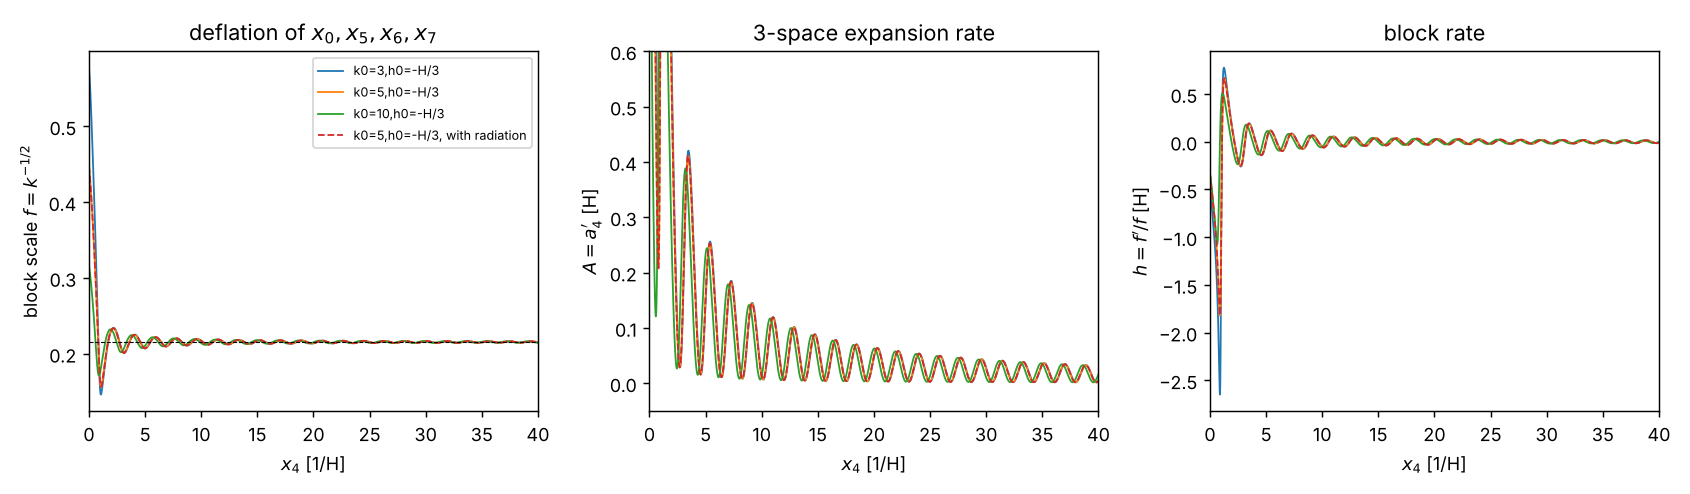
\includegraphics{figures/fig_primordial_history.png}
\caption{Deflation of the extra times into the stabilised block (full
nonlinear Einstein-Lovelock equations with the author's weights).}
\end{figure}

\hypertarget{the-four-dimensional-effective-gravity-derived}{%
\subsection{The four-dimensional effective gravity
(DERIVED)}\label{the-four-dimensional-effective-gravity-derived}}

On a product of a four-dimensional metric with the static block
(constant curvature \(K = -H^2k\)), the Lovelock densities factorise,
\(\mathcal L_{(k)} = \sum_{j+l=k}\frac{k!}{j!\,l!}\mathcal L^{(4)}_{(j)}\mathcal L^{(int)}_{(l)}\)
with \(\mathcal L^{(int)}_{(l)} = (1, 12K, 24K^2, 0)\), and
\(\mathcal L^{(4)}_{(3)} \equiv 0\) in four dimensions while
\(\mathcal L^{(4)}_{(2)}\) (the four-dimensional Gauss-Bonnet density)
is topological. The reduced Lagrangian (gravity plus the stabiliser, in
units of \(1/(2\kappa)\)) is
\[ \sum_k\alpha_k\mathcal L_{(k)} - 2\Lambda - 2\kappa\rho_b = G(k)\,R^{(4)} + (\text{topological}) - 2\,G(k)\,\Lambda_4,\qquad
   \Lambda_4 = \frac{6H^2k(1 - 2w_2k) + \Lambda + \kappa\rho_b}{G(k)} , \]
so the four-dimensional gravity of UM-2 is EXACTLY general relativity
with Newton's constant \(8\pi G_N = \kappa/(G(k_*)V_\perp)\) and the
cosmological term \(\Lambda_4\), which vanishes at the static point by
construction. The observed dark energy is a small residual of this
balance, \(\Lambda_4/H^2 \sim 10^{-92}\): tuned (the
cosmological-constant problem, OPEN).

\hypertarget{dirac16complex-in-the-cell-kohn-sham-description}{%
\section{dirac16complex in the cell: Kohn-Sham
description}\label{dirac16complex-in-the-cell-kohn-sham-description}}

\(\Psi\) is quantised canonically with \(x_4\) as the time,
\(\{\Psi_r(x), \Psi_s^\dagger(x')\} = B_{rs}\,\delta^7(x - x')/\sqrt{|g|}\)
on a slice (\(r, s\) spinor indices); the indefinite Krein metric \(B\)
is handled in the good sector by counting the positive branch of every
block as particles (the record's convention, ASSUMED). The interacting
many-body state is described by Kohn-Sham theory: orbitals of \(h_j\)
with the mean fields
\[ M_{eff}(y) = m + \tfrac{15}{16}\lambda S(y) + \delta M_{portal}(y),\qquad v(y) = -\tfrac{1}{16}\lambda\,n(y) + v_{portal}(y), \]
\[ e_{int} = \tfrac{15}{32}\lambda S^2 - \tfrac{1}{32}\lambda n^2,\qquad E_{KS} = \sum g f\varepsilon - 2\,\mathrm{Vol}_7\!\int_{-L}^{0}\!e^{3Hy}e_{int}\,dy ,\]
where \(n\) and \(S = \bar\Psi\Psi\) are the proper densities,
\(g = 4r_3(n^2)\) the degeneracy of the momentum shell
\(\vec k = \Delta k\,\vec n\) (\(\vec n \in \mathbb Z^3\), \(r_3(n^2)\)
the number of representations of \(n^2\) as a sum of three squares,
\(\Delta k = 0.25H\)), \(\mathrm{Vol}_7 = (2\pi/\Delta k)^3v_tf^4\) the
proper seven-volume of the cell, \(f\) the occupations (aufbau or
Mermin), and the portal mean fields come from I11 (the fermion
densities), I12 (the gluon condensate) and I9 (the \(Z\) charge at the
tip, on \(\Psi_A\) only). The energy-momentum tensor of a Kohn-Sham
state,
\[ \rho = \sum wgf\varepsilon\,n_o - e_{int},\qquad p_3 = \sum wgf\,\tfrac{e^{-a_4}|k|}{3}t_o + e_{int},\qquad p_t = e_{int},\]
\[ p_0 = \sum wgf\big[(\varepsilon - v)n_o - M_{eff}s_o - e^{-a_4}|k|t_o\big] + e_{int} , \]
with \(n_o = P\chi^\dagger\chi\), \(s_o = P\chi^\dagger j\sigma_2\chi\),
\(t_o = P\chi^\dagger j\sigma_3\chi\), \(P = e^{-3Hy}/\mathrm{Vol}_7\)
and \(w = 1/2\), is the source of \(\Psi\) in the gravitational
equations; its block-averaged pressure \((p_0 + 3p_t)/4\) pushes on the
block (section 8.1).

\hypertarget{neutrinos-psi_a-the-z-invisible-width-n_eff-and-the-cnb-derived}{%
\section{\texorpdfstring{Neutrinos, \(\Psi_A\), the \(Z\) invisible
width, \(N_{eff}\) and the CNB
(DERIVED)}{Neutrinos, \textbackslash Psi\_A, the Z invisible width, N\_\{eff\} and the CNB (DERIVED)}}\label{neutrinos-psi_a-the-z-invisible-width-n_eff-and-the-cnb-derived}}

With one generation the \(Z\) decays invisibly into \(\nu\bar\nu\) and
into the \(\Psi_A\) fold band (two Weyl species),
\[ N_\nu \equiv \frac{\Gamma_{inv}(Z)}{\Gamma(Z\to\nu\bar\nu)} = 1 + 2r^2,\qquad r = \frac{g_Z(\Psi_A)}{g_Z(\nu)} ;\]
the measured \(N_\nu = 2.9840 \pm 0.0082\) gives
\(r^2 = 0.9920 \pm 0.0041\). The \(\Psi_A\) species then interact with
the plasma like \(\nu_\mu\) and \(\nu_\tau\) of the three-generation
Standard Model and decouple with the neutrinos (\(T \approx 2.6\) MeV,
after the QCD and pion entropy releases; any \(r^2 > 2\times10^{-3}\)
gives the same temperature), so
\[ N_{eff} = 3.044,\qquad T_\nu = T_{\Psi_A} = \Big(\frac{4}{11}\Big)^{1/3}T_{CMB} = 1.945\ \text{K} .\]
The cosmic neutrino background of UM-2 consists of \(\nu_e\) (massive,
0.05 eV, non-relativistic today) and two massless \(\Psi_A\) species,
\(112\ \text{cm}^{-3}\) per species, \(336\ \text{cm}^{-3}\) in all. The
\(\Psi_B\) fold band is never thermalised (no tip coupling, no scalar
density, \(c_V = 0\)) and contributes nothing.

\hypertarget{the-dark-sector}{%
\section{The dark sector}\label{the-dark-sector}}

\textbf{Dark matter (CONDITIONAL candidate).} The lightest odd state of
\(\Psi_B\), a Dirac fermion of mass
\[ M_{DM} = \varepsilon_{DM} = 3.10220\,m = 44.3\ \text{TeV}\qquad (m = H = 14.28\ \text{TeV}), \]
is cold (\(w = 0\) at rest), electrically neutral and \(Z\)-neutral
exactly at tree level (no tip operator reaches \(\Psi_B\)), stable as
long as the fold parity of \(\Psi_B\) is exact (it is a symmetry of
every interaction that reaches \(\Psi_B\)) and \(N_B\) is conserved
(both hold in the good sector). Its hidden wave number carries 90 \% of
\(\varepsilon^2\): its mass is the author's \(x_0\) mechanism in the
Heisenberg sense. A thermal relic through I12 (p-wave annihilation into
\(W^+W^-\), \(ZZ\), \(Z\gamma\), \(\gamma\gamma\), gluon pairs; standard
radiation-dominated freeze-out) needs
\(\langle\sigma v\rangle(x_f) = 1.37\times10^{-25}\) cm\(^3\)/s, below
the s-wave thermal unitarity estimate
\((4\pi/M_{DM}^2)\sqrt{x_f/\pi} = 2.3\times10^{-25}\) cm\(^3\)/s, i.e.
\((8G_g^2 + 3G_W^2 + G_B^2)^{1/2} = (16.6\ \text{TeV})^{-3}\) for the
four-dimensional coefficients of
\(G_i\,\bar\chi\chi F^i_{\mu\nu}F^{i\mu\nu}\) (canonical fields),
\(G_i = \mathcal O\,c_i\,g_i^2/\Lambda_\star^3\) with \(g_i\) the
four-dimensional gauge couplings and
\(\mathcal O = \partial\varepsilon_{DM}/\partial m = 0.7072\) the
response of the dark-matter level to a uniform mass shift (DERIVED,
Hellmann-Feynman); direct detection is far below current limits. The
relic value assumes that the radion oscillation left over from the
deflation does not dominate and dilute the Universe after freeze-out,
i.e.~it is conditional on the solution of the moduli problem (section
14).

\textbf{Dark energy (NOT SUPPORTED).} No positive-energy state of
\(\Psi\) has \(w < 0\) on the static block; a \(\lambda < 0\) condensate
tuned to \(w_0 = -1\) runs away (\(w_a = -6\)) and its energy density
turns negative at \(z = 0.26\). The dark energy of UM-2 is the tuned
residual \(\Lambda_4\).

\hypertarget{cosmology-cmb-cnb-bao}{%
\section{Cosmology: CMB, CNB, BAO}\label{cosmology-cmb-cnb-bao}}

The four-dimensional effective theory is general relativity (section
8.5) with photons, \(\nu_e\), the two \(\Psi_A\) species, baryons, the
\(\Psi_B\) dark matter and \(\Lambda_4\). Its linear perturbations
(order \(\epsilon\)) obey the standard Einstein-Boltzmann equations.
Solved with the Einstein-Boltzmann code CAMB at the Planck 2018 values
of \(\omega_b\), \(\omega_c\), \(\tau\), \(A_s\), \(n_s\) and
\(\theta_*\) (DERIVED): \(H_0 = 67.43\) km/s/Mpc, \(r_{drag} = 147.10\)
Mpc, the TT and EE spectra agree with Planck \(\Lambda\)CDM to
\(2.2\times10^{-4}\) and \(3.7\times10^{-4}\) (\(30 \le \ell \le 2500\);
at most 0.011 of the cosmic variance \(\sqrt{2/(2\ell + 1)}\) of a
single multipole), and the DESI DR2 BAO give \(\chi^2 = 30.3\) for 13
measurements (Planck \(\Lambda\)CDM: 32.6).

\hypertarget{parameters}{%
\section{Parameters}\label{parameters}}

\begin{longtable}[]{@{}
  >{\raggedright\arraybackslash}p{(\columnwidth - 4\tabcolsep) * \real{0.3333}}
  >{\raggedright\arraybackslash}p{(\columnwidth - 4\tabcolsep) * \real{0.3333}}
  >{\raggedright\arraybackslash}p{(\columnwidth - 4\tabcolsep) * \real{0.3333}}@{}}
\toprule\noalign{}
\begin{minipage}[b]{\linewidth}\raggedright
parameter
\end{minipage} & \begin{minipage}[b]{\linewidth}\raggedright
value
\end{minipage} & \begin{minipage}[b]{\linewidth}\raggedright
status
\end{minipage} \\
\midrule\noalign{}
\endhead
\bottomrule\noalign{}
\endlastfoot
\(H\) & 14.28 TeV & DERIVED from \(m_{KK}\), \(\eta\) and \(f_*\) \\
Lovelock weights \(w\), \(\Lambda\) & \((1, 1/32, 1/1152)\), \(-10H^2\)
& AUTHOR \\
\(\eta = HL\) & 3 & ASSUMED (record) \\
\(m = 3HM\) & \(M = 1/3\) (\(m = H\)) & ASSUMED (record) \\
stabiliser law & \(\rho_b \propto f^{-8}\),
\(p_0 = p_t = \rho_b = -p_3\) & ASSUMED \\
\(k_*\), \(f_*\), \(G(k_*)\) & 21.522, 0.21556, 13.808 & DERIVED \\
\(m_r\) & 48.4 TeV & DERIVED \\
\(m_{KK}\) & 121.2 TeV & DERIVED (fit to \(\rho_0 - 1\)) \\
\(\beta_W\), \(\beta_Z\) & 0.011932, 0.015364 & DERIVED (fit;
\(\beta_Z = \beta_W/\cos^2\theta_W\), on-shell angle) \\
\(\kappa_f\); \(c_\nu, c_e, c_u, c_d\) & 1; 18.671, 10.304, 9.545, 9.134
& ASSUMED; DERIVED (fit to the masses) \\
\(m_\nu\) & 0.05 eV & ASSUMED \\
\(r^2\) (I9) & 0.992 & DERIVED (fit to \(N_\nu\)) \\
\(c_V\) (I11) & 0 (benchmark) & ASSUMED \\
I12 coefficients &
\((8G_g^2 + 3G_W^2 + G_B^2)^{1/2} = (16.6\ \text{TeV})^{-3}\) & DERIVED
(relic requirement) \\
\(M_{DM}\) & 44.3 TeV & DERIVED \\
\end{longtable}

\hypertarget{assumptions-open-problems-and-conflicts-with-data}{%
\section{Assumptions, open problems and conflicts with
data}\label{assumptions-open-problems-and-conflicts-with-data}}

\begin{itemize}
\tightlist
\item
  \textbf{ASSUMED}: the regular tip cutoff \(\eta = 3\); the good sector
  and compact extra times; \(m = H\); the block stabiliser and its
  \(f^{-8}\) law; the boundary assignments of the Standard-Model fields;
  the tip sigma field; \(\kappa_f = 1\), \(c_L = -c_R\);
  \(m_\nu = 0.05\) eV; the record's particle convention for the Krein
  metric.
\item
  \textbf{INVENTED}: the portals I9, I11, I12; the oriented part of I9.
\item
  \textbf{OPEN}: the microscopic origin of the stabiliser; the tachyonic
  extra-time modes outside the good sector; the closed time-like curves
  implied by compact extra times; the radion oscillation left over from
  the deflation (ESTIMATE: its Planck-suppressed decay rate
  \(\Gamma = C_r\,m_r^3/(4\pi\bar M_{Pl}^2)\), with
  \(\bar M_{Pl} = 2.435\times10^{18}\) GeV and an order-one coupling
  factor \(C_r\), gives a lifetime of \(0.43\,\text{s}/C_r\) and the
  reheating temperature
  \(T_{RH} = (90/(\pi^2g_*))^{1/4}\sqrt{\Gamma\bar M_{Pl}} = 1.85\sqrt{C_r}\)
  MeV (\(g_* = 10.75\)), below the 4.7 MeV that nucleosynthesis needs
  unless \(C_r > 6.5\): the cosmological moduli problem, which also
  conditions the dark-matter relic); the Kaluza-Klein graviton spectrum
  with the Lovelock corrections; the \(S\) parameter of the Higgsless
  tip; anomalies of the eight-dimensional bulk theory; the cosmological
  constant (\(\Lambda_4\) tuned to \(10^{-92}H^2\)).
\item
  \textbf{CONFLICTS WITH DATA, inherent in the order}: there is no Higgs
  boson while one is observed at 125 GeV; without it the longitudinal
  \(W^+W^-\) scattering violates perturbative unitarity near
  \(\sqrt{8\pi}\,v \approx 1.2\) TeV, far below the Kaluza-Klein modes
  that could restore it; with one generation the total \(Z\) width is
  1.23 GeV against the measured 2.4955 GeV (the \(\mu\), \(\tau\),
  \(s\), \(c\), \(b\) channels are missing), while its invisible part is
  reproduced through the fit of \(N_\nu\).
\end{itemize}

\end{document}
